\documentclass[10pt]{beamer}
\usepackage[T2A]{fontenc}
\usepackage[utf8]{inputenc}
\usepackage[english,russian]{babel}

\usepackage{amssymb,amsfonts,amsmath}
\usepackage{cite,enumerate,float,indentfirst}
\usepackage{graphicx}
\usepackage{hyperref}
% Цвета для гиперссылок
\definecolor{linkcolor}{HTML}{799B03} % цвет ссылок
\definecolor{urlcolor}{HTML}{799B03} % цвет гиперссылок

% \hypersetup{pdfstartview=FitH,  linkcolor=linkcolor,urlcolor=urlcolor, colorlinks=true}
\hypersetup{unicode=true}

\graphicspath{{images/}}
\DeclareGraphicsExtensions{.pdf,.png,.jpg}
\usepackage{graphicx}
\usepackage{colortbl}
\usepackage{xcolor}
\usepackage{ifthen}
\usepackage{subfigure}
\usepackage{amsthm}
\usepackage{listings} % code format pasting
\lstset{language=Mathematica}
\lstset{basicstyle={\sffamily\scriptsize},
    numbers=left,
    numberstyle=\tiny\color{gray},
    numbersep=5pt,
    breaklines=true,
    captionpos={t},
    frame={lines},
    rulecolor=\color{black},
    framerule=0.5pt,
    columns=flexible,
    tabsize=2
}

% Some themes
\usetheme{Hannover}
% \usetheme{Madrid}
\usefonttheme{professionalfonts}

\setbeamercolor{block title}{use=structure,fg=white,bg=structure.fg!75!black}
\setbeamercolor{block body}{parent=normal text,use=block title,bg=block title.bg!10!bg}
\newcommand<>\Alt[2]{{%
    \sbox0{$\displaystyle #1$}%
    \sbox1{$\displaystyle #2$}%
    \alt#3%
        {\rlap{\usebox0}\vphantom{\usebox1}\hphantom{\ifnum\wd0>\wd1 \usebox0\else\usebox1\fi}}%
        {\rlap{\usebox1}\vphantom{\usebox0}\hphantom{\ifnum\wd0>\wd1 \usebox0\else\usebox1\fi}}%
}}

\title[]{Семинар: Асимптотика, разложение функции в ряд Тейлора}
\author[]{Абдуллин Рустам Фаритович}
\institute[НГУ]
{
    \vspace{0.5cm}
    \begin{minipage}{0.6\linewidth}
        \begin{center}
            \scriptsize
            \textbf{ НОВОСИБИРСКИЙ ГОСУДАРСТВЕННЫЙ УНИВЕРСИТЕТ, НГУ}
        \end{center}
    \end{minipage}
}
\date{\today}

\setbeamertemplate{navigation symbols}{}
\begin{document}
    \begin{frame}
        \titlepage
    \end{frame}

    \section*{Outline}
    \begin{frame}
        \tableofcontents
    \end{frame}

    \section{Асимптотика}
    \begin{frame}
        \frametitle{Асимптотическое равенство}
        \begin{block}{Определение 1}
            \small
            Функции $f$ и $g$ называются асимптотически равными $f \sim  g$ на бесконечности,
            если выполнено условие $\displaystyle \lim_{x \to \infty} \frac{f(x)}{g(x)} = 1$.
        \end{block}

        \begin{block}{Определение 2}
            \small
            Функции $f$ и $g$ называются асимптотически равными в точке $x_0$,
            если выполнено условие $\displaystyle \lim_{x \to x_0} \frac{f(x)}{g(x)} = 1$.
        \end{block}
    \end{frame}


    \begin{frame}
        \begin{figure}
            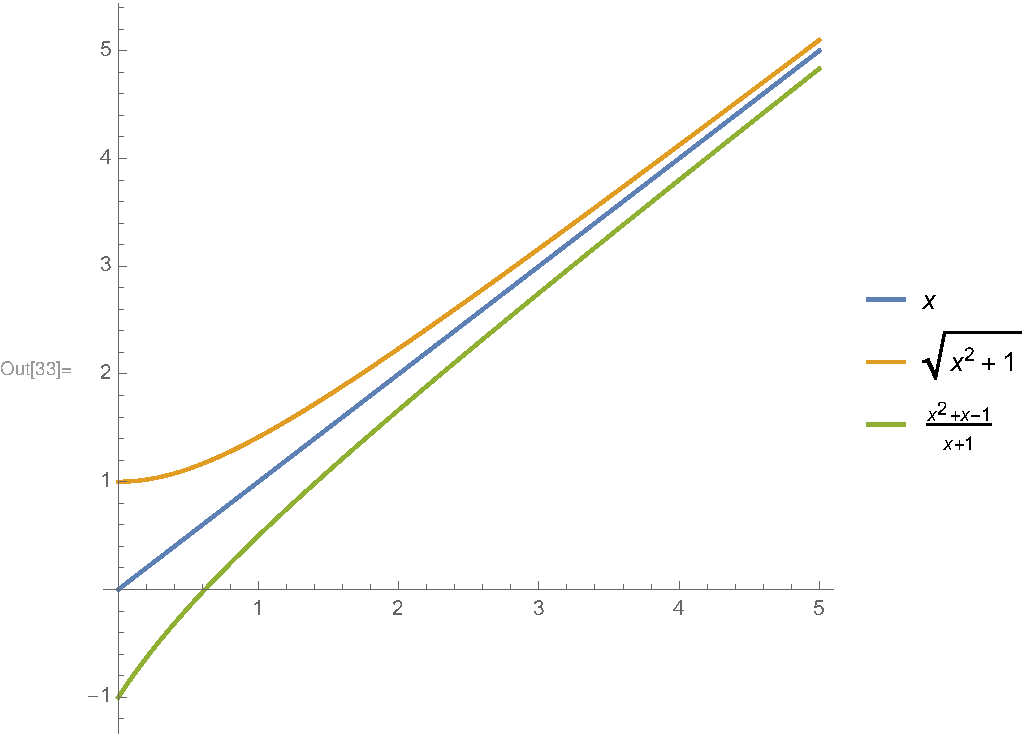
\includegraphics[width = \textwidth]{asymptotic.pdf}
        \end{figure}
    \end{frame}

    \begin{frame}
        \frametitle{Асимптотическое равенство}
        \begin{block}{Определение 3}
            \small
            Функция $f$ есть $O(g)$ (''О''-большое) в точке $x_0$ (на бесконечности),
            если выполнено условие $\displaystyle \lim_{x \to x_0} \frac{f(x)}{g(x)} = C = const$.
        \end{block}

        \begin{block}{Определение 4}
            \small
            Функция $f$ есть $o(g)$ (''o''-малое) в точке $x_0$ (на бесконечности),
            если выполнено условие $\displaystyle \lim_{x \to x_0} \frac{f(x)}{g(x)} = 0$.
        \end{block}
    \end{frame}

    \begin{frame}
        \frametitle{Примеры}
        \textbf{Вычислительная сложность} -- зависимость объёма работы, которая выполняется некоторым алгоритмом, от размера входных данных. 
        Например, сортировка числового массива. Наивный алгоритм имеет сложность $O(n^2)$, быстрые алгоритмы, 
        такие как \textit{MergeSort, QuickSort}, $O(n \log n)$.

        \begin{itemize}
            \item Степенная сложность $T = O(n^m)$ $m$-го порядка
            \item Экспоненциальная сложность $T = O(a^n)$ ($a > 1$)
            \item Полный перебор $T = O(n!) \approx \sqrt{2\pi n}\left(\frac{n}{e}\right)^n$
        \end{itemize}

        Расчет вариантов в шахматных движках имеет экспоненциальную сложность.
    \end{frame}

    \begin{frame}
        \frametitle{Примеры}
        \begin{tabular}{ll}
            $sin(x) = O(x)$ & при $x \to 0$ \\
            $x = o(1)$ & при $x \to 0$ \\
            $x = o(x^2)$ & при $x \to +\infty$ \\
            $\lg x = o(x)$ & при $x \to +\infty$ \\
            $x^n = o(e^x)$ & при $x \to +\infty$
        \end{tabular}
    \end{frame}


    \section{Формула Тейлора}
    \begin{frame}
        \textbf{Многочленом Тейлора} функции $f(x)$, дифференцируемой $k$ раз в точке $x_0$, называют
        \begin{align*}
            T(x) = \sum_{n=0}^k \frac{f^{(n)}(x_0)}{n!}(x-x_0)^n = f(x_0) &+ f'(x_0)(x-x_0) + \ldots + \\ &+ \frac{f^{(k)}(x_0)}{k!}(x-x_0)^k
        \end{align*}

        Легко проверить, что $T^{(n)}(x_0) = f^{(n)}(x_0)$. Можно доказать, что функция $r(x) = |f(x) - T(x)| = o((x-x_0)^k)$. Кратко, это записывается как
        \begin{equation*}
            f(x) = \sum_{n=0}^k \frac{f^{(n)}(x_0)}{n!}(x-x_0)^n + o((x-x_0)^k)
        \end{equation*}
        \textbf{формула Тейлора} с остаточным членом в форме Пеано.
    \end{frame}

    \begin{frame}
        \frametitle{Аппроксимация функций с помощью многочленов}
        Посчитать следующие значения:
        \\
        \begin{tabular}{lll}
            \\
            $\displaystyle \sqrt{3}$  & = & ? \\
            \\
            $\displaystyle \sin{(1)}$ & = & ? \\
            \\
            $\displaystyle e^{\sqrt{2}}$ & = & ?
        \end{tabular}        
    \end{frame}

    \begin{frame}
        \frametitle{Аппроксимация функций с помощью многочленов}
        Посчитать следующие значения:
        \\
        \begin{tabular}{lll}
            \\
            $\displaystyle \sqrt{3}$  & = & $2+\frac{x-4}{4}-\frac{1}{64} (x-4)^2+\frac{1}{512} (x-4)^3-\frac{5 (x-4)^4}{16384}$ \\
            \\
            $\displaystyle \sin{(1)}$ & = & $x-\frac{x^3}{6}$ \\
            \\
            $\displaystyle e^{\sqrt{2}}$ & = & $1+x+\frac{x^2}{2}+\frac{x^3}{6}+\frac{x^4}{24}+\frac{x^5}{120}+\frac{x^6}{720}$
        \end{tabular}        
    \end{frame}

    \begin{frame}
        \frametitle{Аппроксимация функций с помощью многочленов}
        Посчитать следующие значения:
        \\
        \begin{tabular}{lllll}
            \\
            $\displaystyle \sqrt{3}$  &=&  $1.732050808$& $\approx$ & $1.73212$ \\
            \\
            $\displaystyle \sin{(1)}$ &=&  $0.8414709848$& $\approx$ & $0.833333$ \\
            \\
            $\displaystyle e^{\sqrt{2}}$ &=&  $4.113250379$& $\approx$ & $4.11054$ 
        \end{tabular}        
    \end{frame}

\end{document}